\documentclass[12pt, twoside]{article}
\usepackage[letterpaper, margin=1in, headsep=0.5in]{geometry}
\usepackage[english]{babel}
\usepackage[utf8]{inputenc}
\usepackage{amsmath}
\usepackage{amsfonts}
\usepackage{amssymb}
\usepackage{tikz}
\usepackage{yhmath}
%\usetikzlibrary{quotes, angles}

\usepackage{graphicx}
\usepackage{enumitem}
\usepackage{multicol}

\usepackage{fancyhdr}
\pagestyle{fancy}
\fancyhf{}
\renewcommand{\headrulewidth}{0pt} % disable the underline of the header

\fancyhead[RE]{\thepage}
\fancyhead[RO]{\thepage \\ Name: \hspace{3cm}}
\fancyhead[L]{BECA / Dr. Huson / 10th Grade Geometry\\* Unit 6: Analytic geometry\\1 February 2020}

\begin{document}
\subsubsection*{Linear equation under dilation}
  \begin{enumerate}


    \item Plot the line $4x+3y=24$ and the point $D(3,4)$ on the grid below.
    The line is dilated by a factor of 2.\\
    What is the equation of the new line in slope-intercept form?\\
    Regents question:
    \item Jan 2018 \#13\\
    The line whose equation is $3x -5y=4$ is dilated by a scale factor
    of $\frac{5}{3}$ centered at the origin. Which statements are true?\\
    Turn into long true-false problem
      \begin{enumerate}
        \item The image of the line has the same slope as the pre-image but a different $y$-intercept.
        \item The image of the line has the same $y$-intercept as the pre-image but a different slope.
        \item The image of the line has the same $y$-intercept as the pre-image.
        \item The image of the line has a different slope and a different $y$-intercept from the pre-image.
      \end{enumerate}

    \item Jan 2018 \#30\\
    Aliyah says that when the line $4x+3y=24$ is dilated by a scale factor of 2 centered at the point $(3,4)$, the equation of the dilated line is $y=\frac{4}{3}+16$. Is Aliyah correct? Explain why

\subsubsection*{Point-slope applications}
    \item What is an equation of a line which passes through $(6,9)$ and is perpendicular to the line whose equation is $4x-6y=15$?

    \item Given $\overline{AB}$ where $A(1,2)$ and $B(6,-8)$. What is the equation of the perpendicular bisector of $\overline{AB}$?

    \item Given the triangle $ABC$ shown. (graph) What is the equation of the line through $C$ that is perpendicular to $\overline{AB}$? What are the coordinates of $D$, the intersection of $\overline{AB}$ and the altitude through $C$?

    \item Prove that quadrilateral $ABCD$ is a rectangle by calculating the slope of each side and showing that consecutive sides are perpendicular.

    \item Aug 2018 \#35\\
    The vertices of quadrilateral MATH have coordinates M(4,2), A(1,-3), T(9,3), and H(6,8). Prove that quadrilateral MATH is a parallelogram.
    (scaffold)
      \begin{enumerate}
        \item Find four slopes, starting with: $\displaystyle m_{MA}=\frac{-3-2}{1-4}=$
        \item Make two statements about parallel sides:\\
        $ m_{MA} = m_{TH}$ \emph{iff} $\rule{2cm}{0.015mm} \parallel \rule{2cm}{0.015mm}$ %\vspace{2cm}
        \item Conclusion: $MATH$ is a parallelogram because both pairs of opposite sides are $\rule{3cm}{0.015mm}$
    \end{enumerate}

\subsubsection*{Skills review}
  \item Write down the slope perpendicular to the given slope.\\
  $m=\frac{1}{2} \hspace{1cm} m_{\perp} = $

  \item Turn into true-false\\
  Which equation represents a line that is perpendicular to the line represented by (equation)?\\
  (various linear equations)

  \item Write down the missing length of the triangle’s sides.
  $(3,4,5; 6,8,10; 5,12,13; 7, 24, 25)$ data-driven variable inputs?

  \item Write the reason justifying the following statement made in a proof:\\[0.5cm]
  $\overline{DE} \cong \overline{DE} \hspace{1cm} \rule{3cm}{0.015cm}$

\subsubsection*{Distance}

  \item Rhombus $STAR$ has vertices $S(-1,2)$4, $T(2,3)$, $A(3,0)$, and $R(0,-1)$. What is the perimeter of rhombus $STAR$?

\subsubsection*{Equation of a circle}
  \item The point $P(-5,12)$ is on a circle centered at the origin, as shown below.
  \begin{multicols}{2}
    \raggedcolumns
    \begin{enumerate}
      \item Find the radius of the circle. \vspace{3cm}
      \item Write down the equation of the cirle using the form $(x-a)^2+(y-b)^2=r^2$.
    \end{enumerate}
      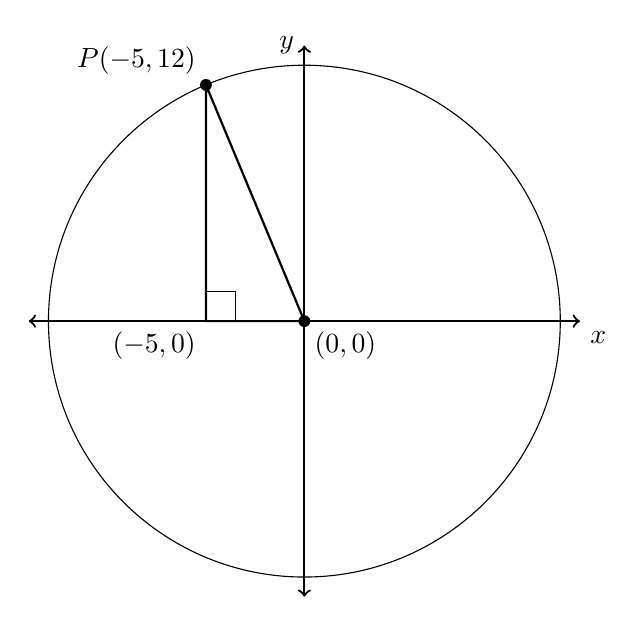
\begin{tikzpicture}[scale=.25]
        \draw [thick, <->] (-14,0) -- (14,0) node [below right] {$x$};
        \draw [thick, <->] (0,-14)--(0,14) node [left] {$y$};
        \draw (0,0) circle[radius=13];
        \draw [thick]
          (-5,0) node[below left] {$(-5,0)$}--
          (0,0) node[below right] {$(0,0)$}--
          (-5,12) node[above left] {$P(-5,12)$}--cycle;
          \fill (0,0) circle[radius=.3];
          \fill (-5,12) circle[radius=.3];
        %\draw [dashed] (0,0)--(-13,0);
        \draw (-5,0) ++(1.5,0)--++(0,1.5)--++(-1.5,0);
      \end{tikzpicture}
  \end{multicols}

  \item What is the equation of a circle with center $(-3,7)$ and radius $r=4$?\vspace{1.5cm}

  \item %June 2018
  What is an equation of circle O shown in the graph below?
  \begin{center}
    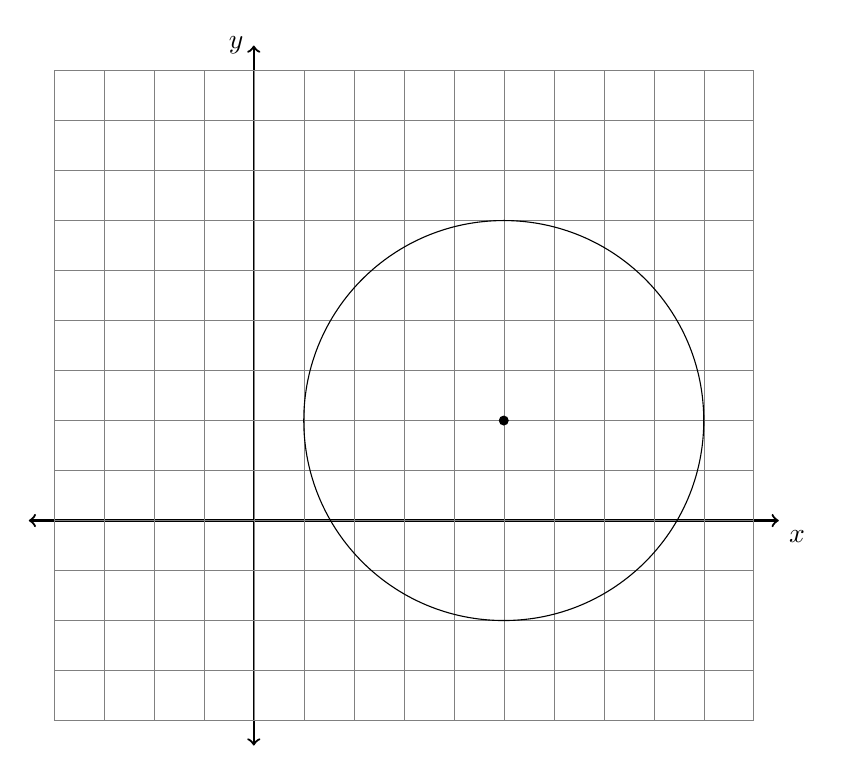
\begin{tikzpicture}[scale=.635]
      \draw [thick, <->] (-4.5,0) -- (10.5,0) node [below right] {$x$};
      \draw [thick, <->] (0,-4.5)--(0,9.5) node [left] {$y$};
      \draw [help lines] (-4,-4) grid (10,9);
      \draw (5,2) circle[radius=4];
        \fill (5,2) circle[radius=.1];
    \end{tikzpicture}
  \end{center}
  \begin{multicols}{2}
    \begin{enumerate}
      \item $x^2+10x+y^2+4y=-13$
      \item $x^2-10x+y^2-4y=-13$
      \item $x^2+10x+y^2+4y=-25$
      \item $x^2-10x+y^2-4y=-25$
    \end{enumerate}
  \end{multicols}

  


  \item %August 2019
  What are the coordinates of the center and the length of the radius of the circle whose equation is $x^2+y^2=8x-6y+39$?
    \begin{enumerate}
      \item center $(-4,3)$ and radius 64
      \item center $(4,-3)$ and radius 64
      \item center $(-4,3)$ and radius 8
      \item center $(4,-3)$ and radius 8
    \end{enumerate}

\item %June 2019
The equation of a cirle is $x^2+8x+y^2-12y=144$. What are the coordinates of the center and the length of the radius of the circle?
  \begin{enumerate}
    \item center $(4,-6)$ and radius 12
    \item center $(-4,6)$ and radius 12
    \item center $(4,-6)$ and radius 14
    \item center $(-4,6)$ and radius 14
  \end{enumerate}

\item %January 2018
The equation of a cirle is $x^2+y^2-6x+2y=6$. What are the coordinates of the center and the length of the radius of the circle?
  \begin{enumerate}
    \item center $(-3,1)$ and radius 4
    \item center $(3,-1)$ and radius 4
    \item center $(-3,1)$ and radius 16
    \item center $(3,-1)$ and radius 16
  \end{enumerate}

\item %Jan 2019
What is an equation of a circle whose center is (1,4) and diameter is 10?
  \begin{enumerate}
    \item $x^2-2x+y^2-8y=8$
    \item $x^2+2x+y^2+8y=8$
    \item $x^2-2x+y^2-8y=83$
    \item $x^2+2x+y^2+8y=83$
  \end{enumerate}    
     
  \item %August 2018
  The equation of a cirle is $x^2+y^2+4x-8y=-16$. The statement that best describes circle $O$ is the
    \begin{enumerate}
      \item center is $(2,-4)$ and is tangent to the $x$-axis
      \item center is $(2,-4)$ and is tangent to the $y$-axis
      \item center is $(-2,4)$ and is tangent to the $x$-axis
      \item center is $(-2,4)$ and is tangent to the $y$-axis
    \end{enumerate}


  \end{enumerate}
\end{document}
